% Created by tikzDevice version 0.6.2 on 2011-12-19 18:30:51
% !TEX encoding = UTF-8 Unicode
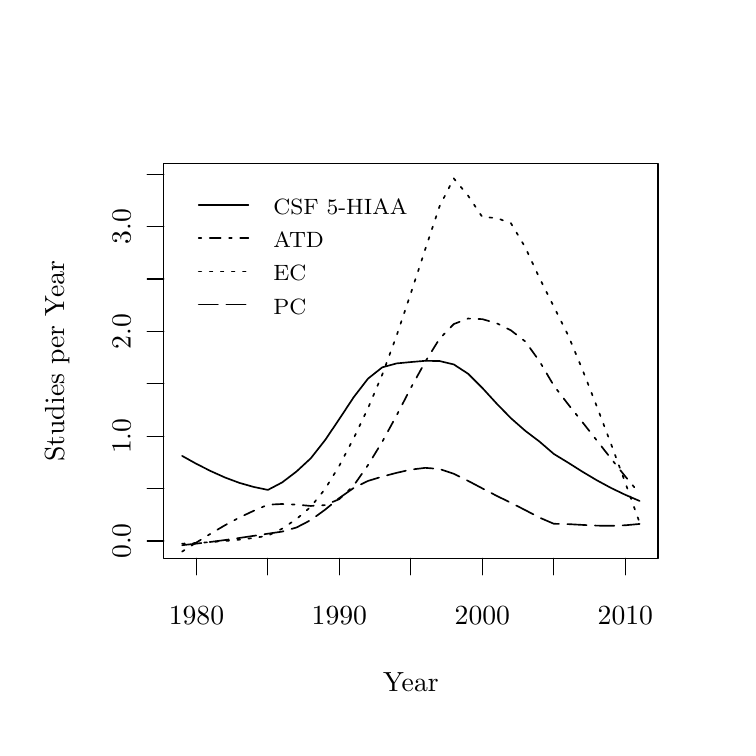
\begin{tikzpicture}[x=1pt,y=1pt]
\definecolor[named]{drawColor}{rgb}{0.00,0.00,0.00}
\definecolor[named]{fillColor}{rgb}{1.00,1.00,1.00}
\fill[color=fillColor,fill opacity=0.00,] (0,0) rectangle (252.94,252.94);
\begin{scope}
\path[clip] ( 49.20, 61.20) rectangle (227.75,203.75);
\definecolor[named]{drawColor}{rgb}{0.00,0.00,0.00}

\draw[color=drawColor,line width= 0.6pt,dash pattern=on 1pt off 3pt ,line cap=round,line join=round,fill opacity=0.00,] ( 55.81, 66.48) --
	( 60.98, 66.74) --
	( 66.15, 67.05) --
	( 71.31, 67.44) --
	( 76.48, 67.93) --
	( 81.64, 68.54) --
	( 86.81, 69.36) --
	( 91.98, 71.93) --
	( 97.14, 75.38) --
	(102.31, 79.81) --
	(107.48, 86.26) --
	(112.64, 94.70) --
	(117.81,104.60) --
	(122.97,115.41) --
	(128.14,127.62) --
	(133.31,141.65) --
	(138.47,157.00) --
	(143.64,172.79) --
	(148.80,188.32) --
	(153.97,198.47) --
	(159.14,192.24) --
	(164.30,184.50) --
	(169.47,184.17) --
	(174.64,182.24) --
	(179.80,173.57) --
	(184.97,162.41) --
	(190.13,152.12) --
	(195.30,141.77) --
	(200.47,129.34) --
	(205.63,116.15) --
	(210.80,102.49) --
	(215.97, 88.45) --
	(221.13, 74.07);
\end{scope}
\begin{scope}
\path[clip] (  0.00,  0.00) rectangle (252.94,252.94);
\definecolor[named]{drawColor}{rgb}{0.00,0.00,0.00}

\draw[color=drawColor,line cap=round,line join=round,fill opacity=0.00,] ( 60.98, 61.20) -- (215.97, 61.20);

\draw[color=drawColor,line cap=round,line join=round,fill opacity=0.00,] ( 60.98, 61.20) -- ( 60.98, 55.20);

\draw[color=drawColor,line cap=round,line join=round,fill opacity=0.00,] ( 86.81, 61.20) -- ( 86.81, 55.20);

\draw[color=drawColor,line cap=round,line join=round,fill opacity=0.00,] (112.64, 61.20) -- (112.64, 55.20);

\draw[color=drawColor,line cap=round,line join=round,fill opacity=0.00,] (138.47, 61.20) -- (138.47, 55.20);

\draw[color=drawColor,line cap=round,line join=round,fill opacity=0.00,] (164.30, 61.20) -- (164.30, 55.20);

\draw[color=drawColor,line cap=round,line join=round,fill opacity=0.00,] (190.13, 61.20) -- (190.13, 55.20);

\draw[color=drawColor,line cap=round,line join=round,fill opacity=0.00,] (215.97, 61.20) -- (215.97, 55.20);

\node[color=drawColor,anchor=base,inner sep=0pt, outer sep=0pt, scale=  1.00] at ( 60.98, 37.20) {1980};

\node[color=drawColor,anchor=base,inner sep=0pt, outer sep=0pt, scale=  1.00] at (112.64, 37.20) {1990};

\node[color=drawColor,anchor=base,inner sep=0pt, outer sep=0pt, scale=  1.00] at (164.30, 37.20) {2000};

\node[color=drawColor,anchor=base,inner sep=0pt, outer sep=0pt, scale=  1.00] at (215.97, 37.20) {2010};

\draw[color=drawColor,line cap=round,line join=round,fill opacity=0.00,] ( 49.20, 67.44) -- ( 49.20,199.98);

\draw[color=drawColor,line cap=round,line join=round,fill opacity=0.00,] ( 49.20, 67.44) -- ( 43.20, 67.44);

\draw[color=drawColor,line cap=round,line join=round,fill opacity=0.00,] ( 49.20, 86.37) -- ( 43.20, 86.37);

\draw[color=drawColor,line cap=round,line join=round,fill opacity=0.00,] ( 49.20,105.31) -- ( 43.20,105.31);

\draw[color=drawColor,line cap=round,line join=round,fill opacity=0.00,] ( 49.20,124.24) -- ( 43.20,124.24);

\draw[color=drawColor,line cap=round,line join=round,fill opacity=0.00,] ( 49.20,143.17) -- ( 43.20,143.17);

\draw[color=drawColor,line cap=round,line join=round,fill opacity=0.00,] ( 49.20,162.11) -- ( 43.20,162.11);

\draw[color=drawColor,line cap=round,line join=round,fill opacity=0.00,] ( 49.20,181.04) -- ( 43.20,181.04);

\draw[color=drawColor,line cap=round,line join=round,fill opacity=0.00,] ( 49.20,199.98) -- ( 43.20,199.98);

\node[rotate= 90.00,color=drawColor,anchor=base,inner sep=0pt, outer sep=0pt, scale=  1.00] at ( 37.20, 67.44) {0.0};

\node[rotate= 90.00,color=drawColor,anchor=base,inner sep=0pt, outer sep=0pt, scale=  1.00] at ( 37.20,105.31) {1.0};

\node[rotate= 90.00,color=drawColor,anchor=base,inner sep=0pt, outer sep=0pt, scale=  1.00] at ( 37.20,143.17) {2.0};

\node[rotate= 90.00,color=drawColor,anchor=base,inner sep=0pt, outer sep=0pt, scale=  1.00] at ( 37.20,181.04) {3.0};

\draw[color=drawColor,line cap=round,line join=round,fill opacity=0.00,] ( 49.20, 61.20) --
	(227.75, 61.20) --
	(227.75,203.75) --
	( 49.20,203.75) --
	( 49.20, 61.20);
\end{scope}
\begin{scope}
\path[clip] (  0.00,  0.00) rectangle (252.94,252.94);
\definecolor[named]{drawColor}{rgb}{0.00,0.00,0.00}

\node[color=drawColor,anchor=base,inner sep=0pt, outer sep=0pt, scale=  1.00] at (138.47, 13.20) {Year};

\node[rotate= 90.00,color=drawColor,anchor=base,inner sep=0pt, outer sep=0pt, scale=  1.00] at ( 13.20,132.47) {Studies per Year};
\end{scope}
\begin{scope}
\path[clip] ( 49.20, 61.20) rectangle (227.75,203.75);
\definecolor[named]{drawColor}{rgb}{0.00,0.00,0.00}

\draw[color=drawColor,line width= 0.6pt,line cap=round,line join=round,fill opacity=0.00,] ( 55.81, 98.20) --
	( 60.98, 95.32) --
	( 66.15, 92.71) --
	( 71.31, 90.39) --
	( 76.48, 88.46) --
	( 81.64, 86.99) --
	( 86.81, 85.91) --
	( 91.98, 88.63) --
	( 97.14, 92.56) --
	(102.31, 97.34) --
	(107.48,103.92) --
	(112.64,111.57) --
	(117.81,119.42) --
	(122.97,126.11) --
	(128.14,130.21) --
	(133.31,131.62) --
	(138.47,132.11) --
	(143.64,132.56) --
	(148.80,132.48) --
	(153.97,131.25) --
	(159.14,127.89) --
	(164.30,122.75) --
	(169.47,117.10) --
	(174.64,111.80) --
	(179.80,107.27) --
	(184.97,103.35) --
	(190.13, 98.90) --
	(195.30, 95.75) --
	(200.47, 92.48) --
	(205.63, 89.41) --
	(210.80, 86.61) --
	(215.97, 84.13) --
	(221.13, 81.91);

\draw[color=drawColor,line width= 0.6pt,dash pattern=on 1pt off 3pt on 4pt off 3pt ,line cap=round,line join=round,fill opacity=0.00,] ( 55.81, 63.63) --
	( 60.98, 66.91) --
	( 66.15, 70.11) --
	( 71.31, 73.15) --
	( 76.48, 75.92) --
	( 81.64, 78.35) --
	( 86.81, 80.57) --
	( 91.98, 80.82) --
	( 97.14, 80.60) --
	(102.31, 80.11) --
	(107.48, 80.42) --
	(112.64, 82.59) --
	(117.81, 87.49) --
	(122.97, 94.86) --
	(128.14,103.33) --
	(133.31,112.82) --
	(138.47,122.79) --
	(143.64,132.17) --
	(148.80,140.50) --
	(153.97,145.84) --
	(159.14,147.83) --
	(164.30,147.61) --
	(169.47,146.14) --
	(174.64,143.55) --
	(179.80,139.55) --
	(184.97,132.37) --
	(190.13,123.57) --
	(195.30,116.84) --
	(200.47,110.38) --
	(205.63,103.81) --
	(210.80, 97.22) --
	(215.97, 90.75) --
	(221.13, 84.58);

\draw[color=drawColor,line width= 0.6pt,dash pattern=on 7pt off 3pt ,line cap=round,line join=round,fill opacity=0.00,] ( 55.81, 65.93) --
	( 60.98, 66.50) --
	( 66.15, 67.12) --
	( 71.31, 67.80) --
	( 76.48, 68.54) --
	( 81.64, 69.31) --
	( 86.81, 70.09) --
	( 91.98, 70.85) --
	( 97.14, 72.33) --
	(102.31, 75.01) --
	(107.48, 78.77) --
	(112.64, 83.00) --
	(117.81, 86.61) --
	(122.97, 89.15) --
	(128.14, 90.73) --
	(133.31, 92.08) --
	(138.47, 93.24) --
	(143.64, 93.88) --
	(148.80, 93.48) --
	(153.97, 91.73) --
	(159.14, 89.18) --
	(164.30, 86.46) --
	(169.47, 83.77) --
	(174.64, 81.24) --
	(179.80, 78.61) --
	(184.97, 75.89) --
	(190.13, 73.67) --
	(195.30, 73.55) --
	(200.47, 73.26) --
	(205.63, 73.00) --
	(210.80, 72.93) --
	(215.97, 73.13) --
	(221.13, 73.61);

\draw[color=drawColor,line width= 0.5pt,line cap=round,line join=round,fill opacity=0.00,] ( 61.77,188.89) -- ( 79.77,188.89);

\draw[color=drawColor,line width= 0.5pt,dash pattern=on 1pt off 3pt on 4pt off 3pt ,line cap=round,line join=round,fill opacity=0.00,] ( 61.77,176.89) -- ( 79.77,176.89);

\draw[color=drawColor,line width= 0.5pt,dash pattern=on 1pt off 3pt ,line cap=round,line join=round,fill opacity=0.00,] ( 61.77,164.89) -- ( 79.77,164.89);

\draw[color=drawColor,line width= 0.5pt,dash pattern=on 7pt off 3pt ,line cap=round,line join=round,fill opacity=0.00,] ( 61.77,152.89) -- ( 79.77,152.89);

\node[color=drawColor,anchor=base west,inner sep=0pt, outer sep=0pt, scale=  1.00] at ( 88.77,185.45) {\footnotesize{CSF 5-HIAA}};

\node[color=drawColor,anchor=base west,inner sep=0pt, outer sep=0pt, scale=  1.00] at ( 88.77,173.45) {\footnotesize{ATD}};

\node[color=drawColor,anchor=base west,inner sep=0pt, outer sep=0pt, scale=  1.00] at ( 88.77,161.45) {\footnotesize{EC}};

\node[color=drawColor,anchor=base west,inner sep=0pt, outer sep=0pt, scale=  1.00] at ( 88.77,149.45) {\footnotesize{PC}};
\end{scope}
\end{tikzpicture}
